\section{Tree-based methods}
\label{sec:Tree-based methods}
\todo{Is boosting a tree method?}
\colorbox{yellow}{Change name of section if boosting is not a tree-based method}\\
In Section~\ref{sec:Linear Classifiers}, only very basic linear methods for classification was discussed. The log odds were modeled in a linear fashion and a decision boundary was drawn based on this. In this section the framework is completely different. The linearity assumptions are removed and the multi class case is considered immediately. 
First, classification trees will be discussed. When this framework is clear, ensemble methods, that try to improve the trees performance, will be presented and compared. This will be done in the following order: Boosting, Bagging and Random forest. 
%
\subsection{Classification trees}
\label{sub:Classification trees}
The idea behind a classification tree is that to make local decisions based on a subset of the predictors. This means that the data is split in subsets, that are again split in new subsets and so on. At the end the subsets are given a class label based on some vote-measure between the data points (usually the majority).
\todo{Always majority?}
This makes the method very general, both in terms of nonlinearity and in type of predictors. The method works with continuous, discrete ordered, and categorical predictors. The tree is also easy to interpret, as one can just follow the splits. For prediction one also just follow the tree down to the decision node, giving the predicted class. There are several different algorithms using this framework. They differ in the methods used for splitting, and in how large to grow the tree. Obviously, growing a full tree, i.e. only one training point in each end node, will cause overfitting, while growing it too short will cause underfitting. This bias-variance tradeoff is important to consider, and there are different methods derived to optimize it. More on the bias-variance tradeoff in appendix~\ref{sub:EPE}. In this \colorbox{yellow}{paper?} only one of the classification tree algorithms will be covered. That is one of the most famous tree methods, proposed by \colorbox{yellow}{reference} \cite{breiman} in 1984, and it is called \textit{Classification And Regression Trees}, or \textit{CART}.
%
\subsubsection{CART}
\label{subsub:CART}
<<cartSim, echo=FALSE>>=
source("../code/cartSim.R")
@
\colorbox{yellow}{This is a special method, not just a general framework}\\
\url{http://stackoverflow.com/questions/9979461/different-decision-tree-algorithms-with-comparison-of-complexity-or-performance}
%
In this section use both \cite{bishop} , \cite{modstat} and \cite{breiman}.

\begin{figure}[h!]
  \centering
  \begin{subfigure}[b]{0.48\textwidth}
    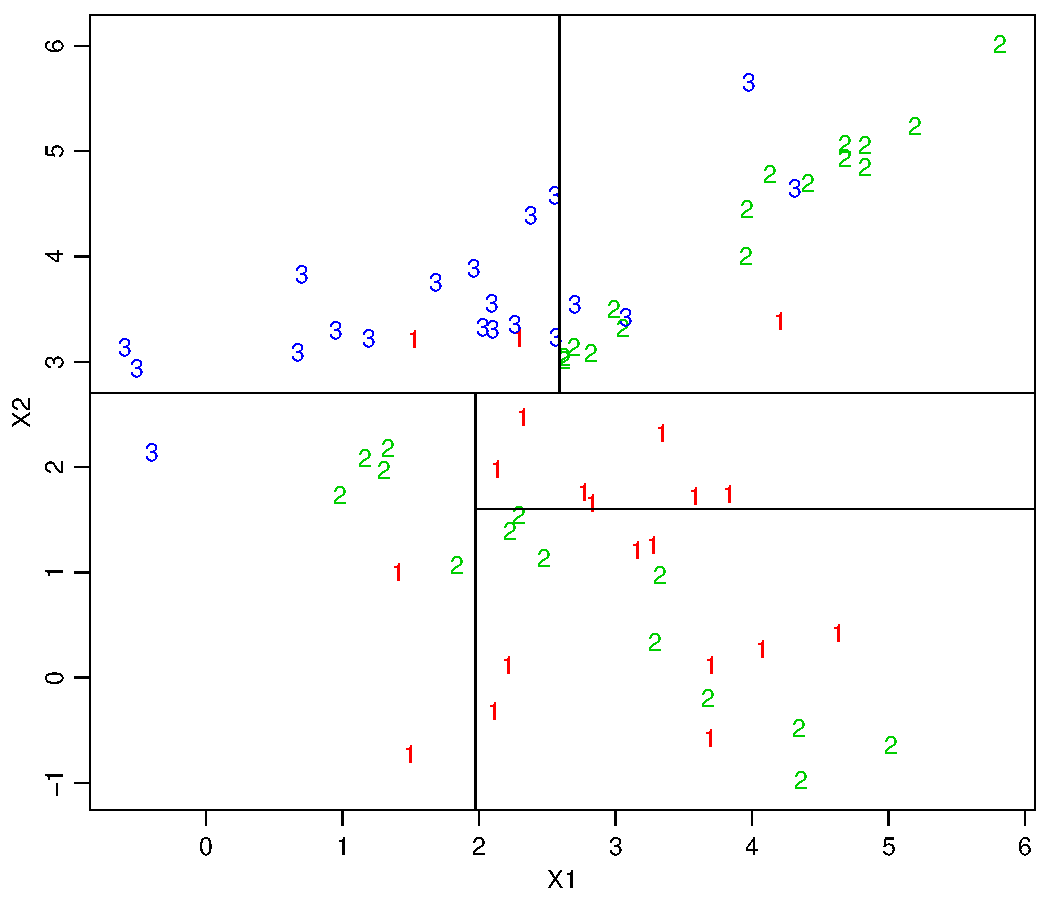
\includegraphics[width=\textwidth]{./figures/cartAreas1.pdf}
    \caption{A gull}
    \label{fig:gull}
  \end{subfigure}%
  \quad
          %(or a blank line to force the subfigure onto a new line)
  \begin{subfigure}[b]{0.48\textwidth}
    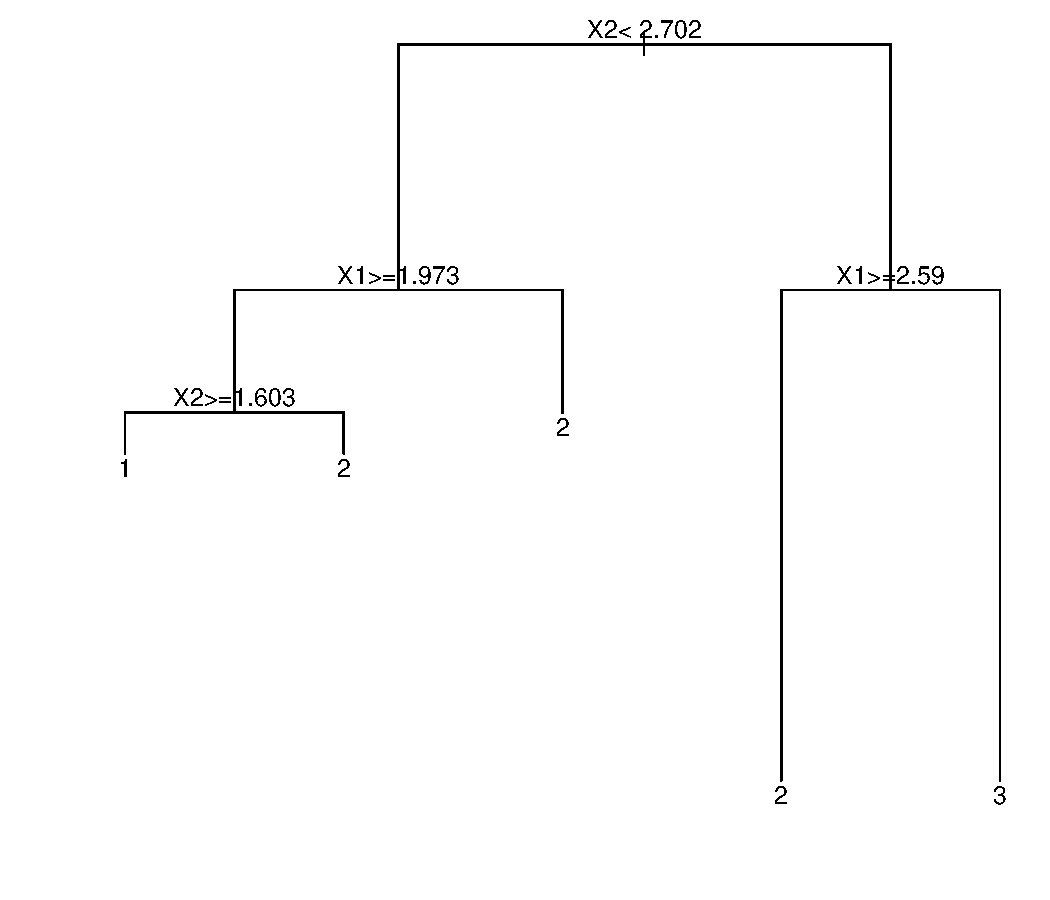
\includegraphics[width=\textwidth]{./figures/cartTree1.pdf}
    \caption{A tiger}
    \label{fig:tiger}
  \end{subfigure}
          %(or a blank line to force the subfigure onto a new line)
  \caption{Pictures of animals}\label{fig:animals}
\end{figure}




\colorbox{yellow}{9.2.4 modstat Other issues: Categorical predictors} \\ \\
%




\subsection{Boosting}
\label{sub:Boosting}

\subsection{Bagging}
\label{sub:Bagging}

\subsection{Random forest}
\label{sub:Random forest}

